\newpage
\genHeader
\hypertarget{validation vis}{} 
\subsection{eMoflon validation support in EA}
\label{sec:EAExport}

Our EA extension provides rudimentary support for validating your metamodel. Validation results are displayed and, in some cases, even ``quick fixes'' to
automatically solve the problems are offered. In addition to reviewing your model, the validation option automatically exports the current model to your eclipse
workspace if no problems were detected.

\begin{stepbystep}
\item If not already active, make the eMoflon control panel visible in EA by choosing ``Extensions/\-Add-In Windows''. This should
display a new output window, as depicted in \Cref{ea:validation_output}.
Many users prefer this interface as it provides quick access to all of eMoflon's features, as opposed to the drop down menu under ``Extensions/MOFLON::Ecore Addin" which only offers limited functionality.

\begin{figure}[htbp]
	\centering
  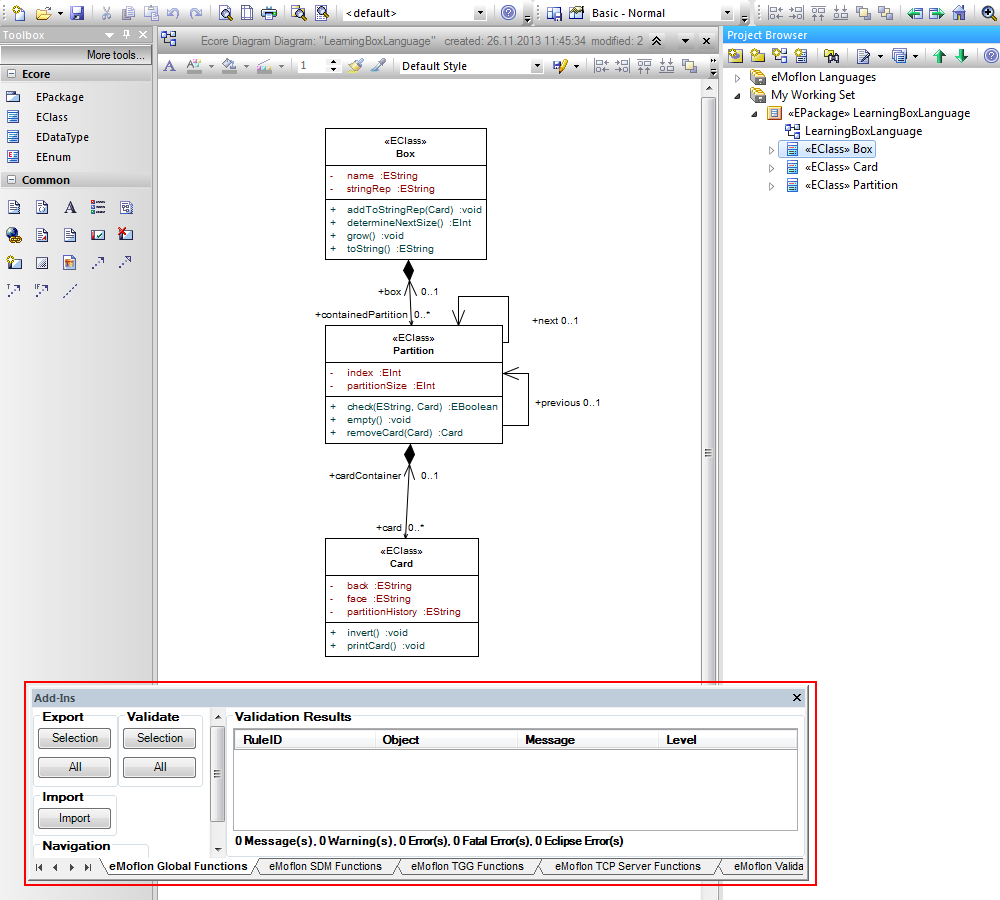
\includegraphics[width=\textwidth]{ea_controlPanel}
	\caption{Activating the validation output window}
	\label{ea:validation_output}
\end{figure}
\FloatBarrier

\clearpage
\item To start the validation, choose ``Validate all'' in the ``Validate" section of the control panel
(\Cref{ea:validation_menu}). If you haven't made any mistakes while modelling your \texttt{LearningBoxLanguage} so far, the validation results window
should remain empty, indicating your metamodels are free of errors.

\begin{figure}[htbp]
	\centering
  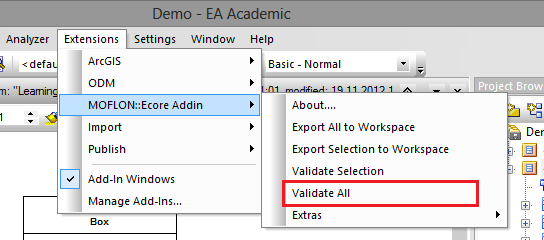
\includegraphics[width=1.0\textwidth]{ea_startValidation}
	\caption{Starting the validation}
	\label{ea:validation_menu}
\end{figure}
\FloatBarrier
\end{stepbystep}

If an error did appear, the validation system attempts to suggest a ``Quick Fix.'' Why don't we examine the validation and quick fix features in detail? Let's
add two small modelling errors in \texttt{LearningBoxLanguage}.

\begin{stepbystep}
\item Create a new EClass in the \texttt{Learning\-Box\-Language} diagram. You can retain the default name \texttt{EClass1}. Let's
assume you wish to delete this class from your metamodel.

\item Select the rouge class in the diagram and press the \texttt{Delete} button on your keyboard. Note that this only deleted it from
the current diagram and \texttt{EClass1} still exists in the project browser (and thus in your metamodel).

\item Run the validation test, and notice the new \texttt{Information} message in the validation output.
%(\Cref{ea:validation_information}).
%
%\begin{figure}[htbp]
%	\centering
%	%TODO lkliegel
%  	%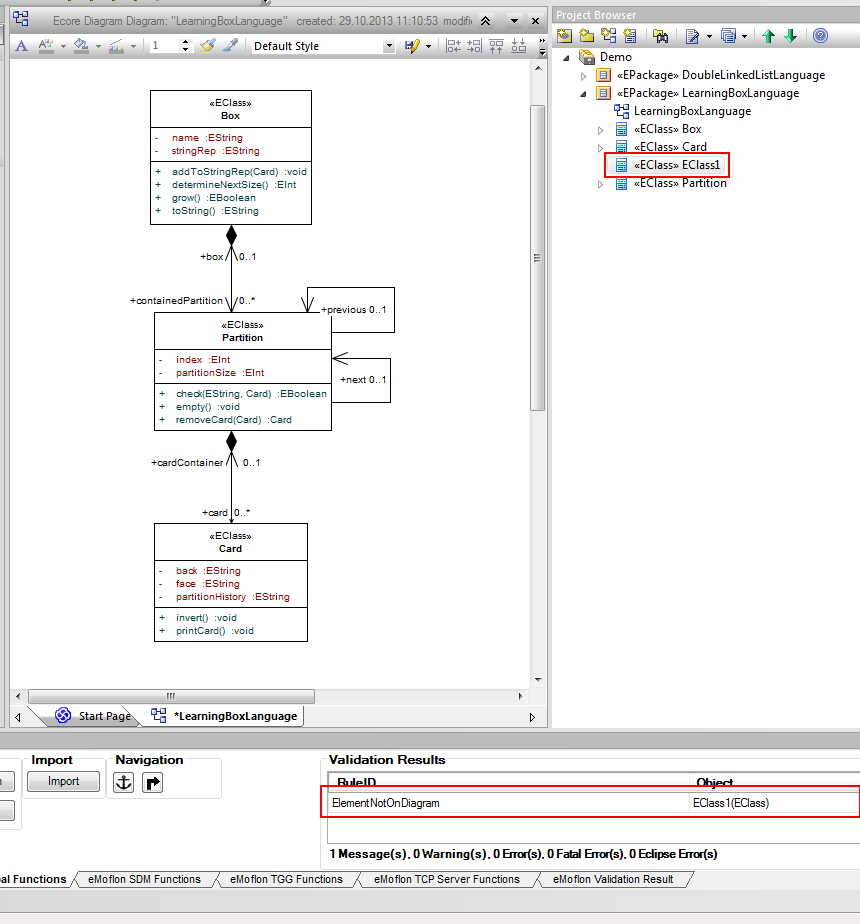
\includegraphics[width=1.0\textwidth]{EA_validationDeleteElement}
%	\caption{Validation information error: element still exists}
%	\label{ea:validation_information}
%\end{figure}

This message informs you that \texttt{EClass1} is not on any diagram, and seeing as it is still in the metamodel, that this \emph{could} be a mistake. As you
can see, just pressing the \texttt{Delete} button is not the proper way of removing an EClass from a metamodel - It only removes it from the current
diagram!\footnote{Deleting elements properly and other EA specific aspects are discussed in detail in Part VI: Micellaneous}

\item Suppose you were inspecting a different diagram, and were not on the current screen. To navigate to the problematic element in the
\texttt{Project Browser}, click \emph{once} on the information message.

\item To check to see if there are any quick fixes available, \emph{double}-click the information message to invoke the ``QuickFix''
dialogue. In this case, there are two potential solutions - add the element to the current diagram or (properly) delete the element from the metamodel
(\Cref{ea:quick-fix1}). Since the latter was the original intent, click \texttt{Ok}.

\vspace{0.5cm}

\begin{figure}[htbp]
	\centering
  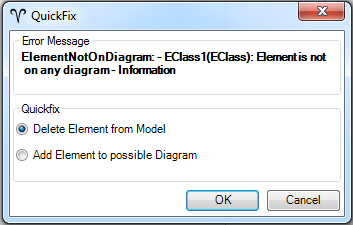
\includegraphics[width=0.55\textwidth]{ea_quickFixElements}
	\caption{Quick fix for elements that are not on any diagram}
	\label{ea:quick-fix1}
\end{figure}
\FloatBarrier

\vspace{0.5cm}

\item \texttt{EClass1} should now be correctly removed from your metamodel. Your metamodel should now be error-free again as indicated by
the validation output window.

\item To make an error that leads to a more critical message than ``information,'' double-click the navigable EReference end
\texttt{previous} of the EClass \texttt{Partition}, and delete its role name as depicted in \Cref{ea:delete-role-name}. Affirm with \texttt{OK}.

\begin{figure}[htbp]
    \centering
  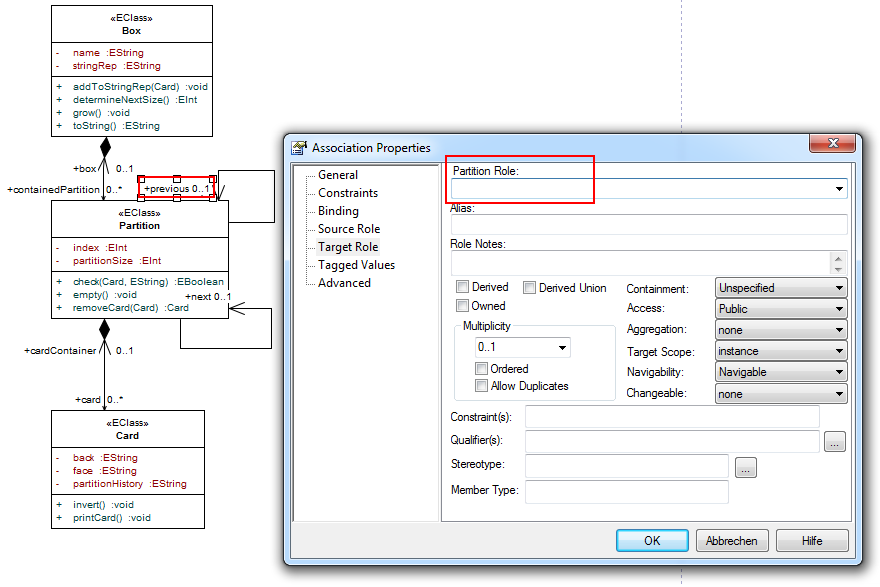
\includegraphics[width=1.0\textwidth]{EA_validationDeleteRoleName}
    \caption{Deleting a navigable role name of an EReference}
    \label{ea:delete-role-name}
\end{figure}

\item You should now see a new \texttt{Fatal Error} in the validation output, stating that a navigable end \emph{must} have a role name.
Close all windows, then single click on the error once to open the relevant diagram and highlight the invalid element on the diagram. Double click the error to
view the quick fix menu (\Cref{ea:fatal-error}). As navigable references are mapped to data members in a Java class, omitting the name of a navigable
reference makes code generation impossible (data members ,i.e., class variables, must have a name).

\begin{figure}[htbp]
	\centering
  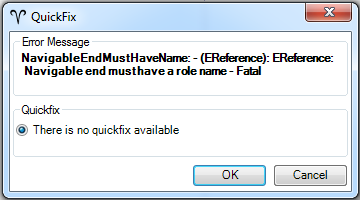
\includegraphics[width=0.6\textwidth]{EA_quickFixFatal}
	\caption{Fatal error after deleting a navigable role name}
	\label{ea:fatal-error}
\end{figure}

\item Given there are no automatic solutions, correct your metamodel manually by setting the name of the navigable EReference back to
\texttt{previous}.

\item Ensure that your metamodel closely resembles \Cref{ea:metamodel_complete} again, and that there are no error messages before
proceeding.

\end{stepbystep}

\vspace*{1cm}

As you may have noticed, eMoflon distinguishes between five different types of validation messages:
\begin{description}
  \item[Information:]~\\
  This is only a hint for the user and can be safely ignored if you know what you're doing.
  Export and code generation should be possible, but certain naming/modelling conventions are violated, or a problematic situation has been detected.
  
  \item[Warning:]~\\ Export and code generation is possible, but only with defaults and automatic corrections applied by the code generator.
  As this might not be what the user wants, such cases are flagged as warnings (e.g., omitting the multiplicity at references which is automatically set by the
  code generator to 1).
  Being as explicit as possible is often better than relying on defaults.
  
  \item[Error:]~\\ Although the metamodel can be exported from EA, it is not Ecore conform, and code generation will not be possible.
 
  \item[Fatal Error:]~\\ The metamodel cannot be exported as required information, such as names or classifiers of model elements is incorrectly set or
  missing.
  
  \item[Eclipse Error:]~\\ Display error messages produced by our Eclipse plugin after an unsuccessful attempt to generate code. 

\end{description}
